%md->tex->template
\documentclass[12pt]{article}
\usepackage{CJKutf8}
\usepackage{amsmath}
\usepackage{geometry}
\usepackage{fancyhdr}
\usepackage{longtable,booktabs}
\usepackage{enumerate}
\usepackage{enumitem}
\usepackage{amsthm}
\usepackage{amssymb}
\usepackage{tikz}
\setlist[enumerate,1]{font=\bfseries}
\geometry{left=3.0cm,right=2.0cm,top=3.0cm,bottom=3.0cm}

\newenvironment{firstlayer}%
{\begin{list}{}{\renewcommand{\makelabel}[1]{\textbf{##1}.\hfil}
}}
{\end{list}}
\newenvironment{secondlayer}%
{\begin{list}{}{\renewcommand{\makelabel}[1]{(##1)\hfil}
}}
{\end{list}}

\renewcommand{\proofname}{\textbf{证明}}

\providecommand{\sol}{\textbf{解}.~}

\title{第 12 次作业}
\author{Log Creative}
\date{May 30, 2020}
\begin{document}

\begin{CJK}{UTF8}{gbsn}

\maketitle

\begin{firstlayer}
  \item[39]对下列集合的整除关系画出哈斯图。
  \begin{secondlayer}
    \item[1] $\{1,2,3,4,6,8,12,24\}$
    
    \sol
    
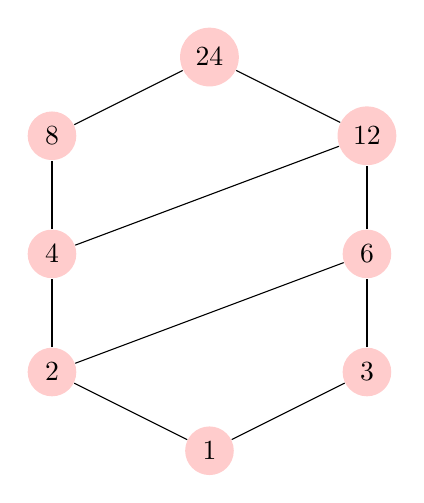
\begin{tikzpicture}

\node[circle, fill=red!20] (v8) at (-0.5,2.5) {24};
\node[circle, fill=red!20] (v9) at (1.5,1.5) {12};
\node[circle, fill=red!20] (v7) at (-2.5,1.5) {8};
\node[circle, fill=red!20] (v5) at (1.5,0) {6};
\node[circle, fill=red!20] (v6) at (-2.5,0) {4};
\node[circle, fill=red!20] (v4) at (1.5,-1.5) {3};
\node[circle, fill=red!20] (v2) at (-2.5,-1.5) {2};
\node[circle, fill=red!20] (v1) at (-0.5,-2.5) {1};
\draw  (v1) edge (v2);
\draw  (v1) edge (v4);
\draw  (v4) edge (v5);
\draw  (v2) edge (v6);
\draw  (v2) edge (v5);
\draw  (v6) edge (v7);
\draw  (v7) edge (v8);
\draw  (v6) edge (v9);
\draw  (v9) edge (v8);
\draw  (v5) edge (v9);
\end{tikzpicture}
  \end{secondlayer}
  \item[42] 设$\mathbf{Z}_+=\{x|x\in \mathbf{Z}\wedge x>0\}$,$D$是$\mathbf{Z}_+$上的整除关系,$T=\{1,2,\cdots,10\}\subseteq \mathbf{Z}_+$。在偏序集$\langle \mathbf{Z}_+,D \rangle$中,求$T$的上界、下界、上确界、下确界。

\sol

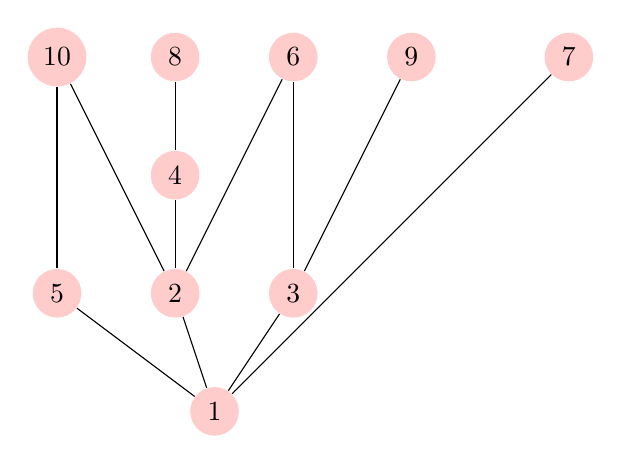
\begin{tikzpicture}

\node[circle, fill=red!20] (v10) at (-1.5,1.5) {10};
\node[circle, fill=red!20] (v8) at (3,1.5) {9};
\node[circle, fill=red!20] (v9) at (5,1.5) {7};
\node[circle, fill=red!20] (v7) at (0,1.5) {8};
\node[circle, fill=red!20] (v5) at (1.5,1.5) {6};
\node[circle, fill=red!20] (v3) at (-1.5,-1.5) {5};
\node[circle, fill=red!20] (v6) at (0,0) {4};
\node[circle, fill=red!20] (v4) at (1.5,-1.5) {3};
\node[circle, fill=red!20] (v2) at (0,-1.5) {2};
\node[circle, fill=red!20] (v1) at (0.5,-3) {1};
\draw  (v1) edge (v2);
\draw  (v1) edge (v3);
\draw  (v1) edge (v4);
\draw  (v4) edge (v5);
\draw  (v2) edge (v6);
\draw  (v2) edge (v5);
\draw  (v6) edge (v7);

\draw  (v1) edge (v9);
\draw  (v4) edge (v8);
\draw  (v3) edge (v10);
\draw  (v2) edge (v10);
\end{tikzpicture}

下界与下确界为1。

上确界为6,7,8,9,10的最小公倍数:2520。

上界为$2520n(n\in \mathbf{Z}_+)$。
\item[46] 对集合$A$,下列的$R$都是$P(A)\times P(A)$上的关系。$R$是否是偏序关系,$R$是否是全序关系。
\begin{secondlayer}
  \item[1]$\langle P,Q\rangle R\langle X,Y\rangle \Leftrightarrow (P \oplus Q)\subseteq (X \oplus Y)$

\sol 自反性成立:
\begin{align*}
&\langle P,Q\rangle R\langle P,Q\rangle \\ 
&\Leftrightarrow (P \oplus Q)\subseteq (P \oplus Q)
\end{align*}

反对称性不成立:\begin{align*}
          &(\langle P,Q\rangle R\langle X,Y\rangle)\wedge(\langle X,Y\rangle R\langle P,Q\rangle) \\
          &\Leftrightarrow (((P \oplus Q)\subseteq (X \oplus Y))\wedge ((X \oplus Y)\subseteq (P \oplus Q))) \\
          &\Leftrightarrow P \oplus Q=X \oplus Y\\
          &\Leftrightarrow (P-Q)\cup(Q-P)=(X-Y)\cup(Y-X)\\
          &\nRightarrow (P=X)\wedge(Q=Y)\\
          &\Rightarrow \langle P,Q\rangle=\langle X,Y\rangle
        \end{align*}

反对称性应当保证两者同时成立时,两个对象相等。

所以不是偏序关系。

不是全序关系:取$A\neq \varnothing:\langle P,Q\rangle=\langle A,\varnothing \rangle,\langle X,Y\rangle = \langle \varnothing,A\rangle$
\begin{align*}
&\langle P,Q\rangle R\langle X,Y\rangle\\
&\Leftrightarrow \langle A,\varnothing \rangle R\langle \varnothing,A\rangle\\
&\Leftrightarrow (A \oplus \varnothing)\subseteq (\varnothing \oplus A)\\
&\Leftrightarrow A\subseteq A\\
&=\text{T}
\end{align*}

\begin{align*}
&\langle X,Y\rangle R\langle P,Q\rangle\\
&\Leftrightarrow \langle \varnothing,A\rangle R\langle A,\varnothing \rangle\\
&\Leftrightarrow (\varnothing \oplus A)\subseteq (A \oplus \varnothing) \\
&\Leftrightarrow A\subseteq A\\
&=\text{T}
\end{align*}

但是$A\neq \varnothing,\langle P,Q\rangle\neq \langle X,Y\rangle$
\end{secondlayer}
\end{firstlayer}


\end{CJK}

\end{document}

